% 专题二：不等式
\section{专题二：不等式}

\begin{learnobjective}
\begin{itemize}
  \item 说出不等关系的来源，会用作差法比较大小；
  \item 会用解集 $S=\{x\in D\mid f(x)>0\}$ 统一求解、证明、存在、最值与参数五类问题；
  \item 会用比较法、分析法证明简单不等式；
  \item 会从函数、极值、几何多个角度重新看待同一个不等式问题；
  \item 会用线性规划处理简单的二元最值问题。
\end{itemize}
\end{learnobjective}

\begin{preview}
\subsection{导语：同一个问题，多个看法}
同一个不等式问题，在不同的知识阶段会有不同的解法。比如“$a^2+b^2$ 与 $2ab$ 谁大”：
初中用完全平方公式，高中用基本不等式，学完二次函数可以用判别式，
学完导数可以用单调性与极值，学到线性规划还能画成图。
本专题把三个“种子问题”用六个视角各做一遍——不是为了多学六种方法，
而是为了看到它们其实是同一件事。

\key{第一层统一}：几乎所有一元不等式都能归结为同一个问题——
\[
  f(x)>0\ \text{在什么地方成立？}
\]
\key{第二层统一}：按“问题目标”分类（求解、证明、存在、无解、最值、参数），
比按表达式类型分类（一次、二次、分式、指数……）更重要：
前者可以用同一套数学语言描述，后者只是外形不同。

\subsection{种子问题}
先自己做，再看后面的六个视角。
\begin{enumerate}
  \item 设 $a,b\in\mathbb{R}$，证明 $a^2+b^2\geq 2ab$，并说明等号成立的条件。
  \item 设 $x>0$，$y>0$，且 $x+y=1$，求 $\dfrac{1}{x}+\dfrac{1}{y}$ 的最小值。
  \item 解不等式 $x^2-2x-3<0$。
\end{enumerate}
\end{preview}

\begin{explore}
\subsection{视角一：统一框架——解集 $S$ 与问题分类}

\key{要点}
\begin{itemize}
  \item 核心对象：设函数 $f$ 的定义域为 $D$，称
  \[
    S=\{x\in D\mid f(x)>0\}
  \]
  为不等式的\key{解集}。一元不等式问题都可以围绕 $S$ 展开（遇到 $<$、$\leq$ 时，改写成 $f(x)<0$、$f(x)\leq0$ 即可）。
  \item 按\key{问题目标}分类：
  \begin{itemize}
    \item 求解型：求 $S$；
    \item 证明型（恒成立）：$S=D$；
    \item 存在型（有解）：$S\neq\varnothing$；
    \item 无解型：$S=\varnothing$；
    \item 最值型：求 $f$ 的最值，用来确定 $S$ 的边界；
    \item 参数型：求参数，使 $S$ 满足某种关系。
  \end{itemize}
  \item 加入条件集合 $A\subseteq D$：
  \[
    \forall x\in A,\ f(x)>0\iff A\subseteq S,\qquad
    \exists x\in A,\ f(x)>0\iff A\cap S\neq\varnothing.
  \]
\end{itemize}

\begin{example}
设 $f(x)=x^2-4x+3=(x-2)^2-1$。同一个函数可以提出五类不同的问题：
\begin{enumerate}
  \item \key{求解}：$f(x)\leq0$ 的解集；
  \item \key{证明}：证明 $f(x)\geq-1$ 对任意实数 $x$ 恒成立；
  \item \key{最值}：求 $f(x)$ 的最小值；
  \item \key{参数（恒成立）}：求 $a$，使 $\forall x\in[1,3],\ f(x)\leq a$；
  \item \key{参数（存在）}：求 $a$，使 $\exists x\in[1,3],\ f(x)\leq a$。
\end{enumerate}
\end{example}
\begin{solution}
$f$ 开口向上，顶点 $(2,-1)$，与 $x$ 轴交于 $1$ 和 $3$。
\begin{enumerate}
  \item $f(x)\leq0\iff (x-1)(x-3)\leq0\iff x\in[1,3]$；
  \item $f(x)+1=(x-2)^2\geq0$，故 $f(x)\geq-1$ 对任意 $x\in\mathbb{R}$ 成立；
  \item 由 (2) 且 $f(2)=-1$，得 $\min f(x)=-1$；
  \item 在 $[1,3]$ 上，$f$ 的最大值为 $0$（在 $x=1$、$x=3$ 处取得），故 $a\geq0$；
  \item 在 $[1,3]$ 上，$f$ 的最小值为 $-1$，故 $a\geq-1$。
\end{enumerate}
\end{solution}

\key{关键观察}：这五类问题都只用到 $f$ 的同一张图象——符号（在 $x$ 轴上方还是下方）与最值。
这不是重新发明解题方法，而是为已有方法建立统一的数学结构。

\key{三种基础工具}
\begin{itemize}
  \item \key{等价变形}：每一步变形都要保持解集不变。例如 $\dfrac1x>1$ 不能直接乘 $x$
        （$x$ 可能为负），须移项通分：$\dfrac{1-x}{x}>0\iff 0<x<1$。
  \item \key{函数的符号、零点与单调性}：严格递增保持大小关系，严格递减反转大小关系；
        用单调性之前必须先确定定义域。例如 $2^x>8=2^3\iff x>3$；
        $\log_{1/2}x>2\iff 0<x<\dfrac14$。
  \item \key{非负性与最值}：$A\geq B\iff A-B\geq0$。配方、因式分解、基本不等式、
        放缩法，本质都是构造一个非负表达式。
\end{itemize}

\begin{problem}
判断下列问题的类型（求解 / 证明 / 存在 / 最值 / 参数），并求解：
\begin{enumerate}
  \item 求 $x^2-4x+3>0$ 的解集；
  \item 证明 $x^2-4x+3\geq-1$；
  \item 是否存在 $x$，使 $x^2-4x+3<-5$？
\end{enumerate}
\end{problem}
\begin{solution}
(1) 求解型：$x^2-4x+3>0\iff x<1$ 或 $x>3$，解集为 $(-\infty,1)\cup(3,+\infty)$；
(2) 证明型：$x^2-4x+3+1=(x-2)^2\geq0$；
(3) 存在型：$f$ 的最小值为 $-1>-5$，故不存在这样的 $x$。
\end{solution}

\key{（回头看：种子问题 1、2、3 分别属于哪一类问题？）}

\subsection{视角二：来源——不等关系从哪来}

\key{要点}
\begin{itemize}
  \item 实数可以比较大小：对任意两个实数 $a,b$，$a-b$ 的符号唯一确定（正、负、零），这就是作差法的依据。
  \item 不等式的基本性质：对称性 $a>b\iff b<a$；传递性 $a>b,\ b>c\Rightarrow a>c$；
        同向可加 $a>b\Rightarrow a+c>b+c$；同乘正数不变号、同乘负数要变号。
  \item 这些性质是“同解变形”的依据：解不等式时每一步变形都必须保持同解。
\end{itemize}

\begin{example}
比较 $a^2+b^2$ 与 $2ab$ 的大小。
\end{example}
\begin{solution}
作差：$a^2+b^2-2ab=(a-b)^2\geq0$，故 $a^2+b^2\geq2ab$，等号当且仅当 $a=b$。
\key{（回头看：种子问题 1 的来源解法）}
\end{solution}

\begin{problem}
已知 $a>b$，$c<d$，比较 $a-c$ 与 $b-d$ 的大小。
\end{problem}
\begin{solution}
由 $c<d$ 得 $-c>-d$；又 $a>b$，同向相加得 $a-c>b-d$。
\end{solution}

\begin{problem}
比较 $x^2+3$ 与 $2x$ 的大小。
\end{problem}
\begin{solution}
$x^2+3-2x=(x-1)^2+2>0$，故 $x^2+3>2x$（对任意实数 $x$ 成立）。
\end{solution}

\subsection{视角三：证明——把“显然”变成“严格”}

\key{要点}
\begin{itemize}
  \item \key{比较法}：作差（判号）或作商（与 $1$ 比，注意两数正负）。
  \item \key{分析法}：从结论出发，逐步寻找充分条件，直到归结为已知事实（执果索因）。
  \item \key{综合法}：从已知出发，逐步推出结论。
  \item \key{基本不等式}：对 $a>0$，$b>0$，有 $\dfrac{a+b}{2}\geq\sqrt{ab}$，等号当且仅当 $a=b$。
\end{itemize}

\begin{example}
证明：对 $a>0$，$b>0$，$\dfrac{a+b}{2}\geq\sqrt{ab}$。
\end{example}
\begin{solution}
作差：$\dfrac{a+b}{2}-\sqrt{ab}=\dfrac{(\sqrt a-\sqrt b)^2}{2}\geq0$，得证。
\end{solution}

\begin{example}
证明：对 $a>0$，$b>0$，$\dfrac{1}{a}+\dfrac{1}{b}\geq\dfrac{4}{a+b}$。
\end{example}
\begin{solution}
作差：
\[
  \frac1a+\frac1b-\frac{4}{a+b}
  =\frac{a+b}{ab}-\frac{4}{a+b}
  =\frac{(a+b)^2-4ab}{ab(a+b)}
  =\frac{(a-b)^2}{ab(a+b)}\geq0,
\]
得证。
\end{solution}

\begin{problem}
设 $x>0$，$y>0$，$x+y=1$，求 $\dfrac1x+\dfrac1y$ 的最小值。
\end{problem}
\begin{solution}
由上面的不等式，$\dfrac1x+\dfrac1y\geq\dfrac{4}{x+y}=4$；
当 $x=y=\dfrac12$ 时取等号。故最小值为 $4$。
\key{（回头看：种子问题 2 的证明解法）}
\end{solution}

\begin{problem}
证明：对 $a>0$，$a+\dfrac1a\geq2$。
\end{problem}
\begin{solution}
作差：$a+\dfrac1a-2=\dfrac{a^2-2a+1}{a}=\dfrac{(a-1)^2}{a}\geq0$，得证。
\end{solution}

\subsection{视角四：函数——把不等式看成函数的位置}

\key{要点}
\begin{itemize}
  \item \key{图象观点}：$f(x)>0$ 的解集，就是函数 $y=f(x)$ 的图象在 $x$ 轴上方部分对应的 $x$ 的范围；$f(x)<0$ 同理。
  \item \key{单调性观点}：递增函数可以“脱掉”——$f(x_1)<f(x_2)\iff x_1<x_2$；递减函数则反向。
\end{itemize}

\begin{example}
解不等式 $x^2-2x-3<0$。
\end{example}
\begin{solution}
令 $f(x)=x^2-2x-3=(x-3)(x+1)$，图象开口向上，与 $x$ 轴交于 $-1$ 和 $3$。
在 $x$ 轴下方的部分是两根之间，故解集为 $(-1,3)$。
\key{（回头看：种子问题 3 的函数解法）}
\end{solution}

\begin{example}
解关于 $x$ 的不等式 $ax>b$，其中 $a,b$ 为参数。
\end{example}
\begin{solution}
设 $f(x)=ax$。
\begin{itemize}
  \item $a>0$ 时 $f$ 递增，$f(x)>b=f\left(\dfrac{b}{a}\right)$，故 $x>\dfrac{b}{a}$；
  \item $a<0$ 时 $f$ 递减，故 $x<\dfrac{b}{a}$；
  \item $a=0$ 时不等式化为 $0>b$：若 $b<0$，解集为 $\mathbb{R}$；若 $b\geq0$，解集为 $\emptyset$。
\end{itemize}
\end{solution}

\begin{problem}
解不等式 $\dfrac{2x-1}{x+2}\leq1$。
\end{problem}
\begin{solution}
移项通分：$\dfrac{2x-1}{x+2}-1\leq0\iff\dfrac{x-3}{x+2}\leq0$。
分子零点 $x=3$，分母零点 $x=-2$，符号分布为 $(-2,3]$，故解集为 $(-2,3]$。
\end{solution}

\subsection{视角五：极值——把“恒成立”看成“最值”}

\key{要点}
\begin{itemize}
  \item 二次函数在 $\mathbb{R}$ 上的最值在顶点处取得；在区间上的最值看对称轴与区间的位置（顶点或端点）。
  \item \key{恒成立 $\iff$ 最值}：$f(x)>0$ 恒成立 $\iff f(x)_{\min}>0$；$f(x)<0$ 恒成立 $\iff f(x)_{\max}<0$。
  \item 用极值可以证明不等式：要证 $f(x)\geq0$，只需证 $f(x)_{\min}\geq0$。
\end{itemize}

\key{导数（求极值的一般工具）}
函数 $y=f(x)$ 在 $x_0$ 处的导数 $f'(x_0)$ 是图象在该点切线的斜率。
$f'(x)>0$ 表示图象上升（函数递增），$f'(x)<0$ 表示下降（函数递减），$f'(x)=0$ 的点可能是极值点。
常用公式：$(x^n)'=nx^{n-1}$。

\begin{example}
求证：对任意实数 $a,b$，$a^2+b^2\geq2ab$。
\end{example}
\begin{solution}
视 $a$ 为变量、$b$ 为参数，设 $f(a)=a^2-2ba+b^2$，开口向上，
最小值在 $a=b$ 处取得，$f(b)=0$，故 $f(a)\geq0$，即 $a^2+b^2\geq2ab$。
\key{（回头看：种子问题 1 的极值证法）}
\end{solution}

\begin{example}
设 $x>0$，$y>0$，$x+y=1$，求 $\dfrac1x+\dfrac1y$ 的最小值。
\end{example}
\begin{solution}
由 $y=1-x$（$0<x<1$），$\dfrac1x+\dfrac1y=\dfrac1x+\dfrac1{1-x}=\dfrac{1}{x(1-x)}$。
分母 $x(1-x)$ 在 $x=\dfrac12$ 处取最大值 $\dfrac14$，故原式取最小值 $4$。
\key{（回头看：种子问题 2 的极值解法）}
\end{solution}

\begin{problem}
求函数 $f(x)=x+\dfrac1x$（$x>0$）的最小值。
\end{problem}
\begin{solution}
$f'(x)=1-\dfrac1{x^2}=\dfrac{x^2-1}{x^2}$。
当 $0<x<1$ 时 $f'(x)<0$；当 $x>1$ 时 $f'(x)>0$。
故 $f$ 在 $x=1$ 处取极小值，也是最小值，$f(1)=2$。
于是得到 $x+\dfrac1x\geq2$（$x>0$）。
\end{solution}

\begin{problem}
求 $f(x)=x^2-2x+2$ 在 $[0,3]$ 上的最小值。
\end{problem}
\begin{solution}
对称轴 $x=1\in[0,3]$，最小值为 $f(1)=1$。
\end{solution}

\begin{problem}
用导数求 $f(x)=x^3-3x$ 的极值。
\end{problem}
\begin{solution}
$f'(x)=3x^2-3=3(x-1)(x+1)$。
$x=-1$ 处取极大值 $f(-1)=2$；$x=1$ 处取极小值 $f(1)=-2$。
\end{solution}

\subsection{视角六：几何——线性规划}

\key{要点}
\begin{itemize}
  \item 二元一次不等式 $ax+by\leq c$ 表示直线 $ax+by=c$ 的一侧（半平面）；不等式组表示几个半平面的公共部分，即\key{可行域}。
  \item 目标函数 $z=ax+by$ 表示一族平行直线，$z$ 在可行域上的最值在顶点处取得。
\end{itemize}

\begin{example}
设 $x>0$，$y>0$，$x+y=1$，求 $x^2+y^2$ 的最小值。
\end{example}
\begin{solution}
$x^2+y^2$ 是点 $(x,y)$ 到原点距离的平方。约束 $x+y=1$ 是一条直线，
原点到该直线的距离为 $\dfrac{|0+0-1|}{\sqrt{1^2+1^2}}=\dfrac{\sqrt2}{2}$，
故 $x^2+y^2\geq\dfrac12$，当 $(x,y)=\left(\dfrac12,\dfrac12\right)$ 时取等号。
\key{（与视角五对照：约束相同，目标不同）}
\end{solution}

\begin{example}
画出不等式组 $\begin{cases}x+y\leq1\\ x\geq0\\ y\geq0\end{cases}$ 表示的平面区域，并求 $z=2x+y$ 的最大值。
\end{example}
\begin{solution}
可行域是以 $(0,0)$、$(1,0)$、$(0,1)$ 为顶点的三角形。
$z=2x+y$ 在三个顶点处的值分别为 $0$、$2$、$1$，故最大值为 $2$（在 $(1,0)$ 处取得）。
\end{solution}

\begin{figure}[htbp]
  \centering
  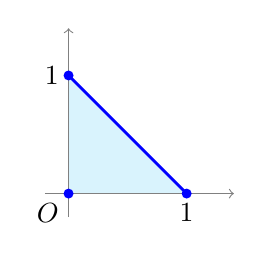
\begin{tikzpicture}[scale=1.5]
    \fill[cyan!15] (0,0) -- (1,0) -- (0,1) -- cycle;
    \draw[->, gray] (-0.2,0) -- (1.4,0);
    \draw[->, gray] (0,-0.2) -- (0,1.4);
    \draw[blue, line width=1pt] (1,0) -- (0,1);
    \fill[blue] (0,0) circle (1.2pt);
    \fill[blue] (1,0) circle (1.2pt);
    \fill[blue] (0,1) circle (1.2pt);
    \node[below] at (1,0) {$1$};
    \node[left] at (0,1) {$1$};
    \node[below left] at (0,0) {$O$};
  \end{tikzpicture}
  \caption{不等式组 $x+y\leq1,\ x\geq0,\ y\geq0$ 表示的可行域}
\end{figure}

\begin{problem}
画出 $\begin{cases}x+y\leq2\\ x\geq0\\ y\geq0\end{cases}$ 表示的区域，并求 $z=x+2y$ 的最大值。
\end{problem}
\begin{solution}
可行域是以 $(0,0)$、$(2,0)$、$(0,2)$ 为顶点的三角形；
$z$ 在顶点处的值为 $0$、$2$、$4$，故最大值为 $4$。
\end{solution}

\key{（回头看：种子问题 2 中 $x+y=1$ 是约束、$\dfrac1x+\dfrac1y$ 是目标；把它画到 $(x,y)$ 平面上，约束是一条直线）}
\end{explore}

\begin{inclasstest}
\subsection{变式训练}
只改一个条件，重新做一遍。
\begin{enumerate}
  \item 证明：对任意实数 $a,b,c$，$a^2+b^2+c^2\geq ab+bc+ca$。
  \item 把种子问题 2 的 $x+y=1$ 改为 $x+y=2$，求 $\dfrac1x+\dfrac1y$ 的最小值。
  \item 把种子问题 3 的 $<0$ 改为 $\geq0$，写出解集；再改为 $x^2-2x-3\geq m$ 恒成立，求 $m$ 的取值范围。
  \item 设 $x>0$，$y>0$，$x+y=1$，求 $x^2+y^2$ 的最小值（与视角六对照）。
  \item 用 $f(x)=x^2-4x+3$ 再设计一个“存在型”问题并求解（与视角一的第 5 题对照）。
\end{enumerate}
\end{inclasstest}

\begin{afterclass}
\subsection{知识来源对照表}
\begin{center}
\footnotesize
\setlength{\tabcolsep}{4pt}
\renewcommand{\arraystretch}{1.35}
\begin{tabular}{p{3.4cm}p{4.0cm}p{5.6cm}}
\toprule
结论 / 方法 & 最早从哪来 & 后面从哪个角度看 \\
\midrule
解集 $S=\{x\mid f(x)>0\}$ & 视角一（统一框架） & 视角二（来源）、视角五（极值） \\
按目标分类 & 视角一（统一框架） & 视角五（极值）、视角六（几何） \\
等价变形 & 视角一（统一框架） & 视角二（来源） \\
作差法 & 视角二（来源） & 视角三（证明）、视角五（极值） \\
平方非负 & 视角二（来源） & 视角三（证明）、视角四（函数） \\
基本不等式 & 视角三（证明） & 视角五（极值）、视角六（几何意义） \\
二次函数图象 & 视角四（函数） & 视角五（极值） \\
恒成立 $\iff$ 最值 & 视角五（极值） & 视角一（统一框架）、视角四（函数） \\
线性规划 & 视角六（几何） & 视角五（约束最值） \\
\bottomrule
\end{tabular}
\end{center}

\key{下一步}：本专题的结构可以复制——换一个主题（如函数与方程、极值），
同样用“种子问题 + 多个视角”重做一遍。
\end{afterclass}
